\section{Поглощающие граничные условия для двумерной системы уравнений акустики} \label{sec:absorbing}

При моделировании волновых процессов в геофизике зачастую приходится иметь дело с неограниченными физическими областями, в которых выделяются конечные расчётные под-области. Волны упругости, выходя за границу такой под-области, продолжают распространяться по неограниченной области, не оказывая влияния на процессы, происходящие внутри расчётной под-области. Для обеспечения такого поведения на практике,  на границах расчётных под-областей необходимо применять специальные условия.

В данной главе будут рассмотрены поглощающие граничные условия Mur и PML для систем уравнений акустики в двумерном случае.

\subsection{Уравнения акустики}


Система уравнений акустики описывает распространение малых колебаний в идеальном газе и является следствием уравнений Эйлера. В двумерном случае она имеет вид

\begin{equation}
\begin{dcases}
	\frac{\partial u}{\partial t} = -\frac{1}{\rho}\frac{\partial p}{\partial x} \\
	\frac{\partial v}{\partial t} = -\frac{1}{\rho}\frac{\partial p}{\partial y} \\
    \frac{\partial p}{\partial t} = -\rho c^2 \left(\frac{\partial u}{\partial x} + \frac{\partial v}{\partial y}\right) \\
\end{dcases}
\label{eq:acoustic}
\end{equation}

Здесь $x$ и $y$ --- координаты в ортонормированной декартовой системе координат, $u(x,y,t)$ и $v(x,y,t)$ --- скорости\footnote{Ранее в \eqref{eq:acoustic_wave_eq} мы обозначали $u\equiv v_x$, $v\equiv v_y$. Здесь переход к новым обозначениям позволяет уменьшить количество индексов, что значительно упрощает запись рассматриваемых далее численных методов.}, $p$ --- давление, $\rho$ --- плотность, $c$ --- скорость звука. Также иногда используют величину $\kappa = \rho c^2$ --- объёмный модуль упругости.

Решение системы будем рассматривать в моменты времени $t \in [0, T]$ в прямоугольной области $\Gamma := \{(x,y) ~|~ (x,y) \in [0, X]\times [0, Y]\}$.

Для краткости записи введём векторную переменную
\begin{equation}
	\varphi = \begin{pmatrix} u \\ v \\ p \end{pmatrix}
\end{equation}

Тогда начальное условие и граничные условия запишутся в следующем виде
\begin{equation}
    \varphi(x,y,0) = \varphi(x,y) ,\qquad (x,y) \in \Gamma
    \label{eq:phi}
\end{equation}
\begin{equation}
\begin{dcases}
    \varphi(0,y,t) = \varphi_L (y,t) , & y \in [0,Y]\\
    \varphi(X,y,t) = \varphi_R (y,t) , & y \in [0,Y]\\
    \varphi(x,0,t) = \varphi_T (x,t) , & x \in [0,X]\\
    \varphi(x,Y,t) = \varphi_B (x,t) , & x \in [0,X]
\end{dcases}
\end{equation}

\subsection{Численное решение системы уравнений акустики}

Здесь и далее решение дискретной задачи будем рассматривать на регулярной прямоугольной сетке с размером шага $h_x$ и $h_y$ соответственно. Для простоты будем считать, что физические размеры рассматриваемой прямоугольной области нацело делятся на шаг сетки: $X=N h_x$, $Y = M h_y$, $N,M \in \mathbb{N}$. Таким образом разностная сетка определяется как $G := \{(x_i, y_j) ~|~ x_i = ih_x, i \in \overline{0,N}, y_j = jh_y, j \in \overline{0,M} \}$. Шаг по времени будем считать постоянным равным $\tau$ и нацело делящим $T$.

При использовании значений в узлах сетки, нижние индексы будем использовать для обозначения пространственных координат, а верхний --- для времени. Например, $p_{i,j}^n$ --- давление в момент времени $t=\tau n \in [0,T]$ в точке с координатами $\left(i h_x, j h_y\right) \in G$ .

\subsubsection{Метод конечных разностей}

Простейшим численным методом решения системы уравнений в частных производных \eqref{eq:acoustic} является метод конечных разностей. Получим одну из возможных разностных схем. Для этого применим явную двухточечную схему для дискретизации производных по времени и центральную двухточечную схему для дискретизации производных по пространственным переменным.
\begin{gather*}
    \dfrac{\partial f}{\partial t} = \dfrac{f^{n+1}_{i,j} - f^{n}_{i,j}}{\tau} \\
    \dfrac{\partial f}{\partial x} = \dfrac{f^{n}_{i+1,j} - f^{n}_{i-1,j}}{2 h_x} \\
    \dfrac{\partial f}{\partial y} = \dfrac{f^{n}_{i,j+1} - f^{n}_{i,j-1}}{2 h_y}
\end{gather*}

Таким образом мы получим следующую разностную схему (leapfrog scheme)
\begin{equation}
\begin{dcases}
	\frac{u^{n+1}_{i,j} - u^{n}_{i,j}}{\tau} = -\frac{1}{\rho}\frac{p^{n+1/2}_{i+1,j} - p^{n+1/2}_{i-1,j}}{2 h_x} \\
	\frac{v^{n+1}_{i,j} - v^{n}_{i,j}}{\tau} = -\frac{1}{\rho}\frac{p^{n+1/2}_{i,j+1} - p^{n+1/2}_{i,j-1}}{2 h_y} \\
    \dfrac{p^{n+3/2}_{i,j} - p^{n+1/2}_{i,j}}{\tau}= -\rho c^2 \left(\frac{u^{n+1}_{i+1,j} - u^{n+1}_{i-1,j}}{2 h_x} + \dfrac{v^{n+1}_{i,j+1} - v^{n+1t}_{i,j-1}}{2 h_y}\right) \\
\end{dcases}
\label{eq:diff}
\end{equation}

Она имеет второй порядок аппроксимации по пространственным переменным и первый по времени.

\subsubsection{Сеточно-характеристический метод}

Более эффективным методом решения гиперболических систем является сеточно-характеристический метод. В части  \ref{sec:elastic_gcm} уже рассматривался вывод сеточно-характеристического метода для решения упругого волнового уравнения. Проведём этот вывод ещё раз, на этот раз для уравнений акустики.

Перепишем исходную систему \eqref{eq:acoustic} в матричном виде, используя раннее введённую переменную $\varphi$ \eqref{eq:phi} 
\begin{equation}
	\varphi_t = \pmb{A} \varphi_x +  \pmb{B} \varphi_y
\end{equation}

\begin{equation}
	\pmb{A} = 
	\begin{pmatrix}
		0 & 0 & -\frac{1}{\rho} \\
		0 & 0 & 0 \\
		-\rho c^2 & 0 & 0			
 	 \end{pmatrix} \qquad
	\pmb{B} = 
	\begin{pmatrix}
		0 & 0 & 0 \\
		0 & 0 & -\frac{1}{\rho} \\
		0 & -\rho c^2 & 0			
    \end{pmatrix}
\end{equation}

Для решения полученной системы воспользуемся методом расщепления: будем решать систему, делая шаг по $x$ на первом полушаге по времени, и делая шаг по $y$ на втором полушаге по времени:

\begin{equation}
\begin{gathered}
	\varphi_t = \pmb{A} \varphi_x \\
	\varphi_t = \pmb{B} \varphi_y
\end{gathered}
\label{eq:syst_split}
\end{equation} 

Таким образом пересчёт на новой временной слой будет иметь вид
\begin{equation}
\begin{gathered}
		\varphi^{t+\Delta t / 2} = S_x(\Delta t / 2, \varphi^t)\\
		\varphi^{t+\Delta t}     = S_y(\Delta t / 2, \varphi^{t+\Delta t/2})
\end{gathered}
\label{eq:gcm_t_steps}
\end{equation} 

где $\Delta t$ --- величина шага по времени, $S_x$ --- некоторый  оператор шага по $x$, $S_y$ --- шага по $y$.

Заметим, что матрицы $\pmb{A}$ и $\pmb{B}$ раскладываются как произведения

\begin{gather}
		\pmb{A} = \pmb{S}_1^{-1} \pmb{\Lambda}_1 \pmb{S}_1\\
		\pmb{B} = \pmb{S}_2^{-1} \pmb{\Lambda}_2 \pmb{S}_2
\end{gather}

где  $\pmb{\Lambda}_i$ --- диагональные матрицы, составленные из собственных чисел матриц $A$ и $B$
\begin{equation}
	\pmb{S}_1^{-1} = 
	\begin{pmatrix}
		0 & \frac{1}{\rho c} & -\frac{1}{\rho c} \\
		1 & 0 & 0 \\
		0 & 1 & 1			
    \end{pmatrix} \qquad
	\pmb{S}_1 = 
	\begin{pmatrix}
		0 & 1 & 0 \\
		\frac{\rho c}{2} & 0 & \frac{1}{2} \\
		-\frac{\rho c}{2} & 0 & \frac{1}{2}		
 	 \end{pmatrix}
\end{equation}

\begin{equation}
	\pmb{S}_2^{-1} = 
	\begin{pmatrix}
		1 & 0 & 0 \\
		0 & \frac{1}{\rho c} & -\frac{1}{\rho c} \\
		0 & 1 & 1			
 	\end{pmatrix} \qquad
	\pmb{S}_2 = 
	\begin{pmatrix}
		1 & 0 & 0 \\
		0 & \frac{\rho c}{2} & \frac{1}{2} \\
		0 & -\frac{\rho c}{2} & \frac{1}{2}	
 	\end{pmatrix}
\end{equation}

\begin{equation}
	\pmb{\Lambda}_1 = \pmb{\Lambda}_2 = 
	\begin{pmatrix}
		0 & 0 & 0 \\
		0 & -c & 0 \\
		0 & 0 & c				
	\end{pmatrix}
\end{equation}

Так как, как было показано выше, матрицы $\pmb{A}$ и $\pmb{B}$ приводятся к диагональному виду, то поставленная задача является гиперболической.

Домножим уравнения \eqref{eq:syst_split} слева на $\pmb{S}_1$ и $\pmb{S}_2$ соответственно:
\begin{equation}
\begin{gathered} 
	\pmb{S}_1\varphi_t = 
	\pmb{S}_1 \pmb{A} \varphi_x =
	\left(\pmb{S}_1 \pmb{S}_1^{-1}\right)\pmb{\Lambda}_1 \pmb{S}_1 \varphi_x =
	\pmb{\Lambda}_1 \left(\pmb{S}_1 \varphi_x \right) \\
	\pmb{S}_2\varphi_t = 
	\pmb{S}_2 \pmb{B} \varphi_y = 
	\left(\pmb{S}_2 \pmb{S}_2^{-1}\right)\pmb{\Lambda}_2 \pmb{S}_2 \varphi_y =
	\pmb{\Lambda}_2 \left(\pmb{S}_2 \varphi_y \right)
\end{gathered}
\end{equation}

Делая замену $\omega^i =  \pmb{S}_i \varphi$, $i\in\{1,2\}$, и учитывая, что матрицы $\pmb{\Lambda}_i$ диагональные, приходим к двум системам из трёх скалярных независимых уравнений переноса:

\begin{equation}
\begin{gathered} 
	\omega^1_t = \pmb{\Lambda}_1 \omega^1_x\\
	\omega^2_t = \pmb{\Lambda}_2 \omega^2_y
\end{gathered}
\end{equation}

Для решения этих скалярных уравнений будем использовать схему TVD второго порядка с ограничителем superbee. \cite{superbee_scheme}

\subsection{Виды поглощающих граничных условий}

Существует три основных подхода для реализации поглощающих граничных условий \cite{Trefethen1996FiniteDA} \cite{arch_comp_sim}:
\begin{enumerate}
    \item  Введение новых пространственных переменных, которые переводят неограниченную рассматриваемую область в ограниченную. На этот подход можно посмотреть и с <<физической>> стороны, рассматривая дискретизацию неограниченного региона сеткой с бесконечно возрастающим по мере удаления от рассматриваемой под-области шагом сетки.
    \item Анализ соотношений между падающей и отражённой волной и постановка граничного условия соответствующего минимизации отражённой части.
    \item Добавление к рассматриваемой ограниченной области новых граничных слоёв, в которых дополнительно вводится диссипативный член, растущий по мере удаления от рассматриваемой области.
\end{enumerate}

В данной работе мы будем обращаться к последним двум подходам, представленным соответственно граничными условиями Mur и PML.

\subsection{Поглощающие граничное условие Mur}

Рассмотрим одномерное волновое уравнение
\begin{equation}
    \dfrac{\partial^2 u}{\partial x^2} - \dfrac{1}{c^2}\dfrac{\partial^2 u}{\partial t^2} = 0
    \label{eq:1d_wave_eq}
\end{equation}

Это уравнение очевидно является одномерным частным случаем двумерной системы уравнений акустики \eqref{eq:acoustic} при $\varphi(x,y,t) = \varphi(x,t)$.

Разложим \eqref{eq:1d_wave_eq} на два уравнения переноса
\begin{equation}
    \dfrac{\partial u}{\partial x} - \dfrac{1}{c} \dfrac{\partial u}{\partial t} = 0
    \label{eq:left_wave}
\end{equation}
\begin{equation}
    \dfrac{\partial u}{\partial x} + \dfrac{1}{c} \dfrac{\partial u}{\partial t} = 0
    \label{eq:right_wave}
\end{equation}

Уравнение \eqref{eq:left_wave} соответствует волне, идущей влево по оси x, а уравнение \eqref{eq:right_wave} --- идущей вправо.

Пусть рассматриваемая область представляет собой отрезок $\gamma := [0, N h_x]$. Поставим поглощающее граничное условие на правом конце (для левой границы это можно сделать абсолютно аналогично). Чтобы правая граница была поглощающей, или не-отражающей, необходимо, чтобы отсутствовала отражённая волна, распространяющаяся влево. В таком случае, на правой границе должно выполняться только уравнение \eqref{eq:right_wave}, а не полное волновое уравнение \eqref{eq:1d_wave_eq}.

\begin{equation}
    \dfrac{\partial u}{\partial x} = -\dfrac{1}{c} \dfrac{\partial u}{\partial t}
\end{equation}

Для того, чтобы при дискретизации производная по времени и производная по пространственной координате были вычислены в одной точке, будем усреднять разностные производные в моменты времени $n$ и $n+1$, получая таким образом решение в точке $x = \left(N-\frac{1}{2}\right)h_x$, $t=\left(n+\frac{1}{2}\right)\tau$. \cite{arch_comp_sim} \cite{idk_book}
%https://w3.pppl.gov/m3d/1dwave/ln_fdtd_1d.pdf

\begin{equation}
    \dfrac{1}{2} \left(\dfrac{u^n_N - u^n_{N-1}}{h_x} + \dfrac{u^{n+1}_N - u^n_{N-1}}{h_y} \right) = -\dfrac{1}{c} \dfrac{1}{2}\left(\dfrac{u^{n+1}_N - u^n_N}{\tau} + \dfrac{u^{n+1}_{N-1} + u^{n+1}_{N-1}}{\tau} \right)
\end{equation}

Обозначая $r = \dfrac{c \tau}{h_x}$, получаем явное выражение для граничного условия

\begin{equation}
    u^{n+1}_N = u^n_{N-1} + \dfrac{r-1}{r+1}(u^{n+1}{N-1}-u^n_N)
\end{equation}

В одномерном случае поглощающее условие Mur является точным. Распространить его можно и на двухмерный случай для рассматриваемой нами системы уравнений акустики \eqref{eq:acoustic}

\begin{equation}
    u^{n+1}_{N,j} = u^n_{N-1,j} + \dfrac{r-1}{r+1}(u^{n+1}{N-1,j}-u^n_{N,j})
\end{equation}

В этом случае поглощение будет точным только если волна падает строго нормально на рассматриваемую границу, соответствуя тем самым одномерному случаю. В противном случае будет наблюдаться  возникновение отражённых от границы волн.

\subsection{Berenger PML}

Поглощающее граничное условие \textit{perfectly matched layer} (PML) впервые было введено в работе \cite{berenger} для системы уравнений Максвелла, описывающих распространение электромагнитных волн. Оказывается \cite{pml_from_maxwell}, что, произведя необходимые замены переменных, эту систему уравнений можно свести к системе уравнений акустики \eqref{eq:acoustic}.

Для реализации затухания в PML слое добавляются диссипативные слагаемые $c u \sigma_x(x,y)$ и $c u \sigma_y(x,y)$, где в качестве функций $\sigma_{x/y}$ обычно выбирают

\begin{gather}
	\sigma_x = \left(\frac{d_x}{w_{x}}\right)^k \Sigma_{x}\\
	\sigma_y = \left(\frac{d_y}{w_{y}}\right)^k \Sigma_{y}
\end{gather}
    
здесь $d_{x/y}(x,y)$ --- глубина проникновения в PML слой, имеющий глубину $w_{x/y}$, $k$ --- степень скорости роста коэффициентов PML, $\Sigma_{x/y}$ --- максимальные значения диссипативных слагаемых\footnote{Глубина проникновения в PML слой очевидно меньше ширины слоя, а значит множитель перед $\Sigma_{x/y}$ лежит в пределах от 0 до 1. Значит $\sigma_{x/y}$ лежит в пределах от 0 до $\Sigma_{x/y}$.}. 

\begin{figure}[htp]
    \centering
    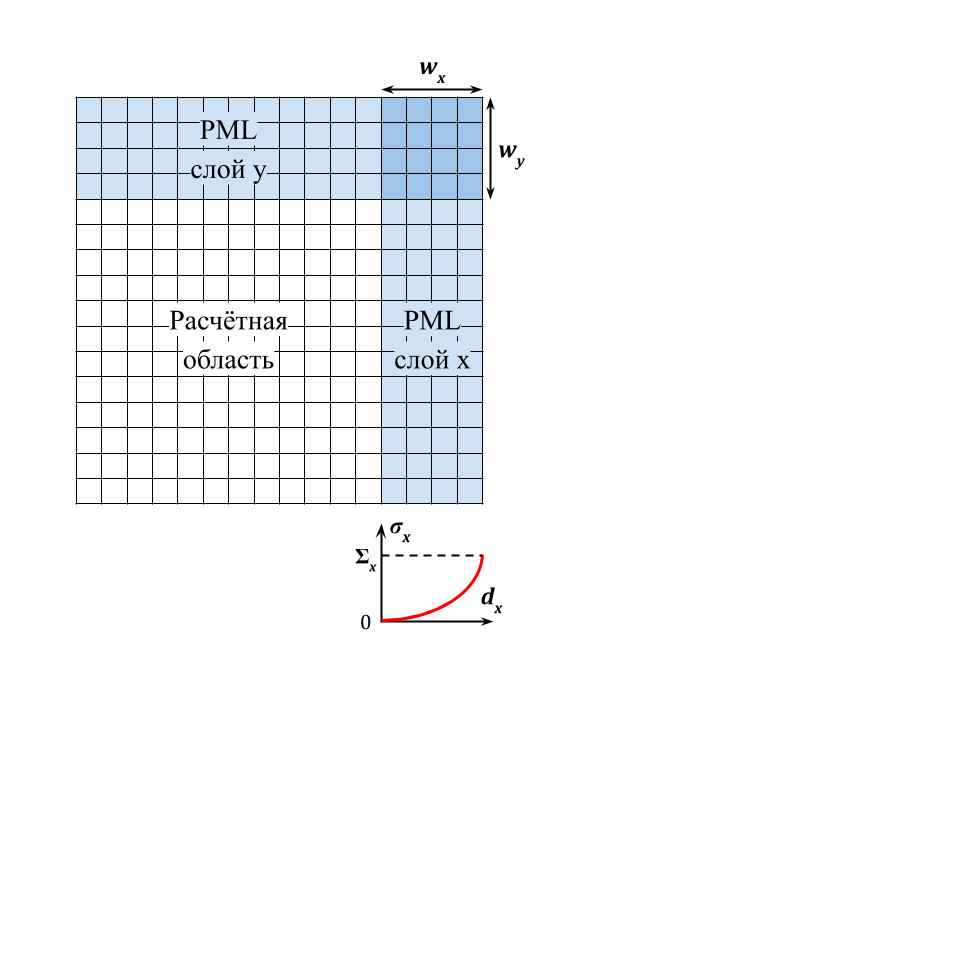
\includegraphics[trim={72pt 325pt 430pt 55pt},clip,width=0.4\textwidth]{images/pml/pml_scheme.png}
    \caption{Схема правого и верхнего PML слоёв.}
    \label{fig:pml_scheme}
\end{figure}

Значения параметров $k$ и $\Sigma_{x,y}$ обычно подбираются под конкретную задачу из эмпирических соображений для наиболее эффективной реализации поглощающего граничного условия.

В случае применения PML на всех четырёх границах прямоугольной области $\Gamma$, то, используя обозначения, введённые для рассчётной сетки $G$, можно записать
    
\begin{gather}
	d_x = h_x \cdot \min\{i, N - i\} \\
	d_y = h_y \cdot \min\{j, M - j\}  
\end{gather}
    
Система уравнений акустики c диссипативными членами имеет вид \cite{pml_from_maxwell}
    
\begin{equation}
	\begin{dcases}
		\frac{\partial u}{\partial t} + c\sigma_x u = -\frac{1}{\rho}\frac{\partial p}{\partial x} \\
		\frac{\partial v}{\partial t} + c\sigma_y u = -\frac{1}{\rho}\frac{\partial p}{\partial y} \\
	    \frac{\partial p}{\partial t} + c(\sigma_x + \sigma_y) p = -\rho c^2 \left(\frac{\partial u}{\partial x}+\frac{\partial v}{\partial y}\right) - \rho c^2 \sigma_x \frac{\partial Q}{\partial y} - \rho c^2 \sigma_y \frac{\partial P}{\partial x} \\
	    \frac{\partial Q}{\partial t} = cv \\
	    \frac{\partial P}{\partial t} = cu
	\end{dcases}\label{eq:pml} 
\end{equation}
    
где $Q$ и $P$ --- дополнительные переменные, определяющиеся из последних двух уравнений.
    
\subsection{Split-field PML}

Другим классическим вариантом граничного условия PML является так называемый \textit{split-field PML} \cite{aaaaaaaaaa}

\begin{equation}
	\begin{dcases}
	    \left(\frac{\partial}{\partial t} + \sigma_x(x)\right) p_1 + \kappa \frac{\partial}{\partial x} v_x = 0 \\
	    \left(\frac{\partial}{\partial t} + \sigma_y(y)\right) p_2 + \kappa \frac{\partial}{\partial y} v_y = 0 \\
	    \left(\frac{\partial}{\partial t} + \sigma_x(x)\right) v_x + \frac{1}{\rho} \frac{\partial}{\partial x} p = 0 \\
	    \left(\frac{\partial}{\partial t} + \sigma_y(y)\right) v_y + \frac{1}{\rho} \frac{\partial}{\partial y} p = 0 \\
	    p = p_1 + p_2
	\end{dcases}\label{eq:split_pml} 
\end{equation}
    
где, напомним,  $\kappa = \rho c^2$ --- объёмный модуль упругости. Функции $\sigma_{x/y}$ выбираются аналогично случаю Berenger PML.

В системе \eqref{eq:split_pml} давление $p$ разделяется на  компоненты $p_1$ и $p_2$. В начальный момент времени они определяются как половины общего значения давления $p$: $p_1(x,y,t=0) = p_2(x,y,t=0) = \frac{p(x,y)}{2}$. В дальнейшем $p_1$ и $p_1$ определяются из численных уравнений, а $p$ вычисляется после каждой итерации, как сумма $p_1$ и $p_2$. 
    
\subsection{Решение PML-систем методом конечных разностей}
    
Аналогично разностной схеме \eqref{eq:diff} для системы уравнений  акустики, заменяя аналитические производные на разностные, получим системы разностных уравнений для Berenger PML \eqref{eq:pml}
    
\begin{equation}
	\begin{dcases}
		\frac{u^{n+1}_{i,j} - u^{n}_{i,j}}{\tau} + c \sigma_{x_{i}} u^{n} = -\frac{1}{\rho}\frac{p^{n+\sfrac{1}{2}}_{i+\sfrac{1}{2},j} - p^{n+\sfrac{1}{2}}_{i-\sfrac{1}{2},j}}{h_x} \\
		\frac{v^{n+1}_{i,j} - v^{n}_{i,j}}{\tau} + c \sigma_{y_{j}} v^{n}  = -\frac{1}{\rho}\frac{p^{n+\sfrac{1}{2}}_{i,j+1} - p^{n+\sfrac{1}{2}}_{i,j-1}}{2h_y} \\
		\frac{Q^{n+1} - Q^{n}}{\tau} = c v^n_{i,j}\\
		\frac{P^{n+1} - P^{n}}{\tau} = c u^n_{i,j}\\
	    \dfrac{p^{n+\sfrac{3}{2}}_{i,j} - p^{n+\sfrac{1}{2}}_{i,j}}{\tau} + c \left(\sigma_{x_{i}} + \sigma_{y_{j}}\right)p^{n+\sfrac{1}{2}} =\\= -\rho c^2 \left(\frac{u^{n+1}_{i+1,j} - u^{n+1}_{i-1,j}}{2h_x} + \dfrac{v^{n+1}_{i,j+1} - v^{n+1}_{i,j-1}}{2h_y} - \sigma_{x_i}\frac{Q^{n+1}_{i,j+1} - Q^{n+1}_{i,j}}{h_y} - \sigma_{y_j}\frac{P^{n+1}_{i+1,j} - P^{n+1}_{i,j}}{h_x} \right)
	\end{dcases}\label{eq:diff_pml}
\end{equation}
    
и для split-field PML \eqref{eq:split_pml}
\begin{equation}
    \begin{dcases}
        (p_1)_{i,j}^{n+1}
        p_{i,j}^{n+1} = (p_1)_{i,j}^{n+1} + (p_2)_{i,j}^{n+1}
    \end{dcases}
    \label{eq:diff_split_pml}
\end{equation}
    
\subsection{Решение PML-систем сеточно-характеристическим методом}
    
Cеточно-характеристический метод, рассмотренный в первой главе, является более эффективным по сравнению с простым конечно-разностным методом. Покажем, что он применим для решения систем уравнений Berenger PML \eqref{eq:pml} и split-field pml \eqref{eq:split_pml}.
    
\subsubsection{Berenger PML}
    
Рассмотрим систему уравнений, реализующую затухающее граничнее условие типа PML \eqref{eq:pml}, и произведём замену:
\begin{equation}
    \varphi = \begin{pmatrix}
        u \\ v \\ p \\ Q \\ P
    \end{pmatrix}
\end{equation}
    
Тогда система принимает вид
\begin{equation}
    \varphi_t = \pmb{A}\varphi_x + \pmb{B}\varphi_y + \pmb{S}\varphi
\end{equation}

где матрицы $\pmb{A}$, $\pmb{B}$ и $\pmb{S}$ следующие
\begin{equation*}
    \pmb{A} = \begin{pmatrix}
        0 & 0 & -\frac{1}{\rho} & 0 & 0 \\
        0 & 0 & 0 & 0 & 0 \\
        -\rho c^2 & 0 & 0 & 0 & -\rho c^2 \sigma_y \\
        0 & 0 & 0 & 0 & 0 \\
        0 & 0 & 0 & 0 & 0
    \end{pmatrix} \qquad
	\pmb{B} = \begin{pmatrix}
        0 & 0 & 0 & 0 & 0 \\
        0 & 0 & -\frac{1}{\rho} & 0 & 0 \\
        0 & -\rho c^2  & 0 & -\rho c^2 \sigma_x & 0 \\
        0 & 0 & 0 & 0 & 0 \\
        0 & 0 & 0 & 0 & 0
    \end{pmatrix}
\end{equation*}
    
\begin{equation*}
	\pmb{S} = \begin{pmatrix}
        -c \sigma_x & 0 & 0 & 0 & 0 \\
        0 & -c \sigma_y & 0 & 0 & 0 \\
        0 & 0 & -c (\sigma_x + \sigma_y) & 0 & 0 \\
        0 & c & 0 & 0 & 0 \\
        c & 0 & 0 & 0 & 0
    \end{pmatrix}
\end{equation*}

Эти матрицы можно диагонализовать

\begin{equation*}
    \pmb{A} = \pmb{L}_1 \pmb{\Lambda}_1 \pmb{R}_1
\end{equation*}
\begin{equation*}
    \pmb{B} = \pmb{L}_2 \pmb{\Lambda}_2 \pmb{R}_2
\end{equation*}
\begin{equation*}
    \pmb{S} =\pmb{L}_3 \pmb{\Lambda}_3 \pmb{R}_3
\end{equation*}


\begin{equation*}
    \pmb{L}_1 = \begin{pmatrix}
        0 & 0 & 1 & 0 & 0 \\
        0 & -\sigma_y & 0 & \frac{1}{c \rho} & -\frac{1}{c \rho} \\
        0 & 0 & 0 & 1 & 1 \\
        0 & 1 & 0 & 0 & 0 \\
        1 & 0 & 0 & 0 & 0
    \end{pmatrix} \qquad
    \pmb{R}_1 = \begin{pmatrix}
        0 & 0 & 0 & 0 & 1 \\
        0 & 0 & 0 & 1 & 0 \\
        1 & 0 & 0 & 0 & 0 \\
        0 & \frac{c \rho}{2} & \frac{1}{2} & \frac{c \rho \sigma_y}{2} & 0  \\
        0 & -\frac{c \rho}{2}  & \frac{1}{2} & - \frac{c \rho \sigma_y}{2} & 0
    \end{pmatrix}
\end{equation*}
    
\begin{equation*}
    \pmb{L}_2 = \begin{pmatrix}
        -\sigma_x & 0 & 0 & \frac{1}{c \rho} & -\frac{1}{c \rho} \\
        0 & 0 & 1 & 0 & 0 \\
        0 & 0 & 0 & 1 & 1 \\
        0 & 1 & 0 & 0 & 0 \\
        1 & 0 & 0 & 0 & 0
    \end{pmatrix} \qquad
    \pmb{R}_2 = \begin{pmatrix}
        0 & 0 & 0 & 0 & 1 \\
        0 & 0 & 0 & 1 & 0 \\
        0 & 1 & 0 & 0 & 0 \\
        \frac{c \rho}{2} & 0 & \frac{1}{2} & 0 & \frac{c \rho \sigma_x}{2}  \\
        -\frac{c \rho}{2} & 0 & \frac{1}{2} & 0 & - \frac{c \rho \sigma_x}{2} 
    \end{pmatrix}
\end{equation*}

\begin{equation*}
    \pmb{\Lambda}_1 = \pmb{\Lambda}_2 = \begin{pmatrix}
        0 & 0 & 0 & 0 & 0 \\
        0 & 0 & 0 & 0 & 0 \\
        0 & 0 & 0 & 0 & 0 \\
        0 & 0 & 0 & -c & 0 \\
        0 & 0 & 0 & 0 & c
    \end{pmatrix} 
\end{equation*}
    

\begin{equation*}
    \pmb{L}_3 = \begin{pmatrix}
        0 & 0 & -\sigma_x & 0 & 0 \\
        0 & 0 & 0 & -\sigma_y & 0 \\
        0 & 0 & 0 & 0 & 1 \\
        0 & 1 & 0 & 1 & 0 \\
        1 & 0 & 1 & 0 & 0
    \end{pmatrix} \qquad
    \pmb{R}_3 = \begin{pmatrix}
        \sigma_x^{-1} & 0 & 0 & 0 & 1 \\
        0 & \sigma_y^{-1} & 0 & 1 & 0 \\
        -\sigma_x^{-1} & 0 & 0 & 0 & 0 \\
        0 & -\sigma_y^{-1} & 0 & 0 & 0 \\
        0 & 0 & 1 & 0 & 0
    \end{pmatrix}
\end{equation*}

\begin{equation*}
    \pmb{\Lambda}_3 = \begin{pmatrix}
        0 & 0 & 0 & 0 & 0 \\
        0 & 0 & 0 & 0 & 0 \\
        0 & 0 & -c \sigma_x & 0 & 0 \\
        0 & 0 & 0 & -c \sigma_y & 0 \\
        0 & 0 & 0 & 0 & -c (\sigma_x + \sigma_y)
    \end{pmatrix}
\end{equation*}

Полученное векторное уравнение в частных производных можно расщепить по физическим процессам для каждой компоненты аналогично уравнению переноса-диффузии с $\mu = 0$ \cite{rashep_marchuk}.

Будем решать систему, делая шаг по $x$ на первой трети шага по времени, делая шаг по $y$ на второй, и решая неоднородное уравнение на третей части шага по времени:
\begin{gather*} 
	\label{eq:pml_eq_split_1} \varphi_t = \pmb{A} \varphi_x \\
	\label{eq:pml_eq_split_2} \varphi_t = \pmb{B} \varphi_y \\
	\label{eq:pml_eq_split_3} \varphi_t = \pmb{S} \varphi
\end{gather*}

Домножая $i$-ое уравнение слева на $\pmb{R_i}$
\begin{gather*} 
    \pmb{R}_1 \varphi_t = \pmb{R}_1\left(\pmb{L}_1 \pmb{\Lambda}_1 \pmb{R}_1\right) \varphi_x \\
	\pmb{R}_2 \varphi_t = \pmb{R}_2\left(\pmb{L}_2 \pmb{\Lambda}_2 \pmb{R}_2\right) \varphi_y \\
	\pmb{R}_3 \varphi_t = \pmb{R}_3\left(\pmb{L}_3 \pmb{\Lambda}_3\pmb{ R}_3\right) \varphi
\end{gather*}
\begin{gather*} 
    \pmb{R}_1 \varphi_t = \pmb{\Lambda}_1 \pmb{R}_1 \varphi_x \\
	\pmb{R}_2 \varphi_t = \pmb{\Lambda}_2 \pmb{R}_2 \varphi_y \\
	\pmb{R}_3 \varphi_t = \pmb{\Lambda}_3 \pmb{R}_3 \varphi
\end{gather*}
    
Делая замену $\omega^i = \pmb{R}_i\varphi $, $i\in\{1,2,3\}$, и учитывая, что матрицы $\pmb{\Lambda}_i$ диагональные, приходим к трём системам из трёх скалярных независимых уравнений:
\begin{equation}
\begin{dcases}
    \omega^1_t = \pmb{\Lambda}_1 \omega^1_x \\
	\omega^2_t = \pmb{\Lambda}_2 \omega^2_y \\
	\omega^3_t = \pmb{\Lambda}_3 \omega^3
\end{dcases}
\label{eq:pml_grid_char_sys}
\end{equation}

Первые две системы представляют собой независимые скалярные уравнения переноса. Для их численного решения мы  воспользуемся TVD-схемой второго порядка с ограничителем superbee.
    
Третья система представляет собой 5 независимых скалярных уравнений с разделяемыми переменными, которые очевидно решаются аналитически. Обозначая номер уравнения нижним индексом $l$, получаем

\begin{equation*}
\begin{dcases}
    \left(\omega^3_l\right)_t = 0 & l=1,2\\
    \left(\omega^3_l\right)_t = \left[\pmb{\Lambda}_3\right]_{ll} \omega^3_l & l=3,4,5
\end{dcases}
\end{equation*}

\begin{equation*}
\begin{dcases}
    \omega^3_l(t) = \omega^3_l(t=0) & l=1,2 \\
    \omega^3_l(t) = \omega^3_l(t=0) \cdot \exp\left(\left[\pmb{\Lambda}_3\right]_{ll} t\right) & l = 3,4,5
\end{dcases}
\end{equation*}

Таким образом построен сеточно-характеристический метод решения уравнения \eqref{eq:pml}.

\subsubsection{Split-Field PML}

Теперь построим сеточно-характеристический метод решения системы уравнений split-field PML \eqref{eq:split_pml}

На этот раз произведём замену
\begin{equation}
	\varphi = \begin{pmatrix} u \\ v \\ p_1 \\ p_2 \end{pmatrix}
\end{equation}

Тогда система принимает вид
\begin{equation}
	\varphi_t = \pmb{A} \varphi_x +  \pmb{B} \varphi_y - \pmb{C} \varphi
\end{equation}
где 
\begin{equation}
	\pmb{A} = 
	\begin{pmatrix}
    	0 & 0 & \frac{1}{\rho} & \frac{1}{\rho} \\
    	0 & 0 & 0 & 0 \\
        \kappa & 0 & 0 & 0 \\
    	0 & 0 & 0 & 0
	\end{pmatrix} \qquad
	\pmb{B} = 
	\begin{pmatrix}
    	0 & 0 & 0 & 0 \\
        0 & 0 & \frac{1}{\rho} & \frac{1}{\rho} \\
    	0 & 0 & 0 & 0 \\
        0 & \kappa  & 0 & 0
	\end{pmatrix} \qquad
	\pmb{C} = 
	\begin{pmatrix}
    	\sigma_x & 0 & 0 & 0 \\
    	0 & \sigma_y & 0 & 0 \\
        0 & 0 & \sigma_x & 0 \\
    	0 & 0 & 0 & \sigma_y
	\end{pmatrix}
\end{equation}

Опять замечаем, что матрицы можно диагонализовать
\begin{gather*}
	\pmb{A} = \pmb{L}_1 \pmb{\Lambda}_1 \pmb{R}_1 = 
	\begin{pmatrix}
    	0 & 0 & -\frac{1}{\sqrt{\kappa\rho}} & \frac{1}{\sqrt{\kappa\rho}} \\
    	0 & 1 & 0 & 0 \\
        -1 & 0 & 1 & 1 \\
    	1 & 0 & 0 & 0
	\end{pmatrix} 
	\begin{pmatrix}
    	0 & 0 & 0 & 0 \\
    	0 & 0 & 0 & 0 \\
        0 & 0 & -\sqrt{\frac{\kappa}{\rho}} & 0 \\
    	0 & 0 & 0 & \sqrt{\frac{\kappa}{\rho}}
	\end{pmatrix} 
	\begin{pmatrix}
    	0 & 0 & 0 & 1 \\
    	0 & 1 & 0 & 0 \\
        -\frac{\sqrt{\kappa\rho}}{2} & 0 & \frac{1}{2} & \frac{1}{2} \\
        \frac{\sqrt{\kappa\rho}}{2} & 0 & \frac{1}{2} & \frac{1}{2}
	\end{pmatrix} \\
	\pmb{B} = \pmb{L}_2 \pmb{\Lambda}_2 \pmb{R}_2 = 
	\begin{pmatrix}
    	0 & 1 & 0 & 0 \\
    	0 & 0 & -\frac{1}{\sqrt{\kappa\rho}} & \frac{1}{\sqrt{\kappa\rho}} \\
    	-1 & 0 & 0 & 0 \\
        1 & 0 & 1 & 1 
	\end{pmatrix} 
	\begin{pmatrix}
    	0 & 0 & 0 & 0 \\
    	0 & 0 & 0 & 0 \\
        0 & 0 & -\sqrt{\frac{\kappa}{\rho}} & 0 \\
    	0 & 0 & 0 & \sqrt{\frac{\kappa}{\rho}}
	\end{pmatrix} 
	\begin{pmatrix}
    	0 & 0 & -1 & 0 \\
    	1 & 0 & 0 & 0 \\
        0 & -\frac{\sqrt{\kappa\rho}}{2} & \frac{1}{2} & \frac{1}{2} \\
        0 & \frac{\sqrt{\kappa\rho}}{2}  & \frac{1}{2} & \frac{1}{2}
	\end{pmatrix} 
\end{gather*}

Опять воспользуемся расщеплением по физическим процессам для каждой компоненты полученного векторного уравнение в частных \cite{rashep_marchuk}. Тогда, расщепляя систему и домножая на $\pmb{L_i}^{-1}=\pmb{R_i}$ слева, получим
\begin{equation}
    \begin{dcases}
        \pmb{R}_1\varphi_t = \pmb{\Lambda}_1\pmb{R}_1 \varphi_x\\
        \pmb{R}_2\varphi_t = \pmb{\Lambda}_2\pmb{R}_2 \varphi_y\\
        \varphi_t = - \pmb{C} \varphi  
    \end{dcases}
\end{equation}

Производя замену переменныx $\omega_i = \pmb{R}_i \varphi$:
\begin{equation}
    \begin{dcases}
        \omega_t^1 = \pmb{\Lambda}_1\omega_x^1 \\
        \omega_t^2 = \pmb{\Lambda}_2\omega_y^2 \\
        \varphi_t = - \pmb{C} \varphi  
    \end{dcases}
\end{equation}

Решение этой системы аналогично уже разобранному решению системы \eqref{eq:pml_grid_char_sys}. 

Таким образом система уравнений split-field PML \eqref{eq:split_pml} также решается сеточно-характеристическим методом.

\subsection{Численные эксперименты}

\begin{equation}
    \kappa(x,y,t) = \dfrac{3}{2} / p(x,y,t) \ dV(x,y)
\end{equation}
\begin{equation}
    K = \dfrac{3}{2} \sum_{i=1}^N \sum_{j=1}^M p(i h_x,j h_y,t) h_x h_y
\end{equation}

\begin{figure}[H]
    \centering
    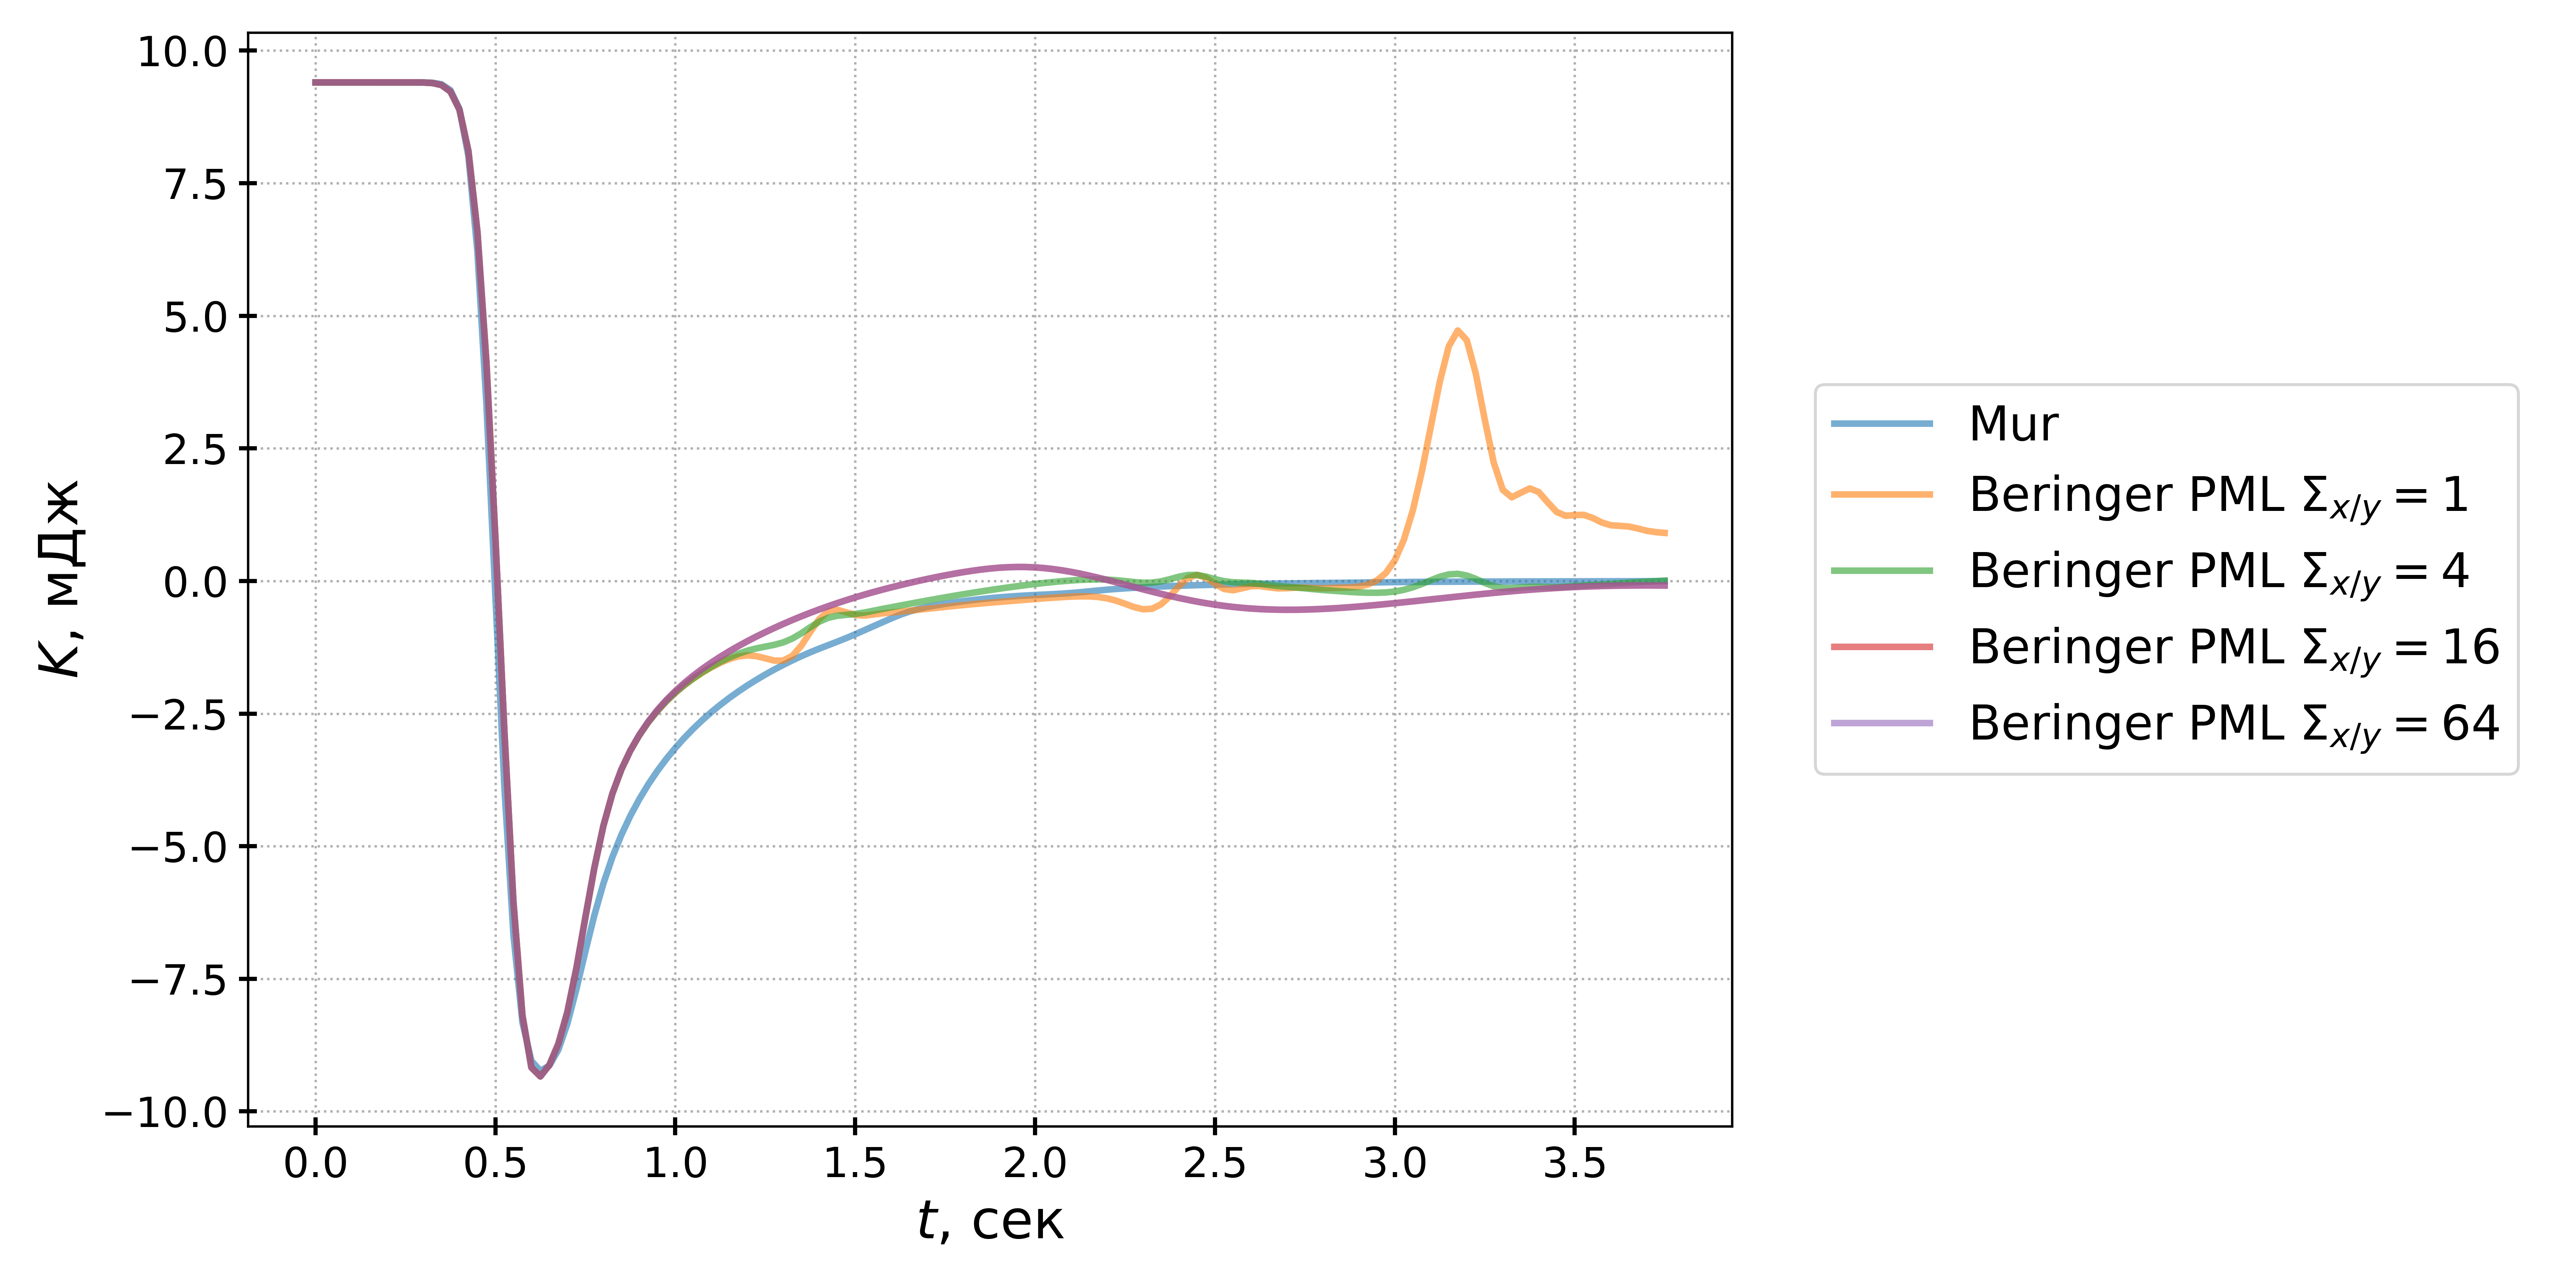
\includegraphics[width=1.0\textwidth]{images/pml/fd_beringer.png}
    \caption{Зависимость кинетической энергии от времени для конечно-разностной реализации поглощающих граничных условий Mur и Berenger PML для различных значений параметра $\Sigma_{x/y}$.}
    \label{fig:fd_Berenger_pml}
\end{figure}

\begin{figure}[H]
    \centering
    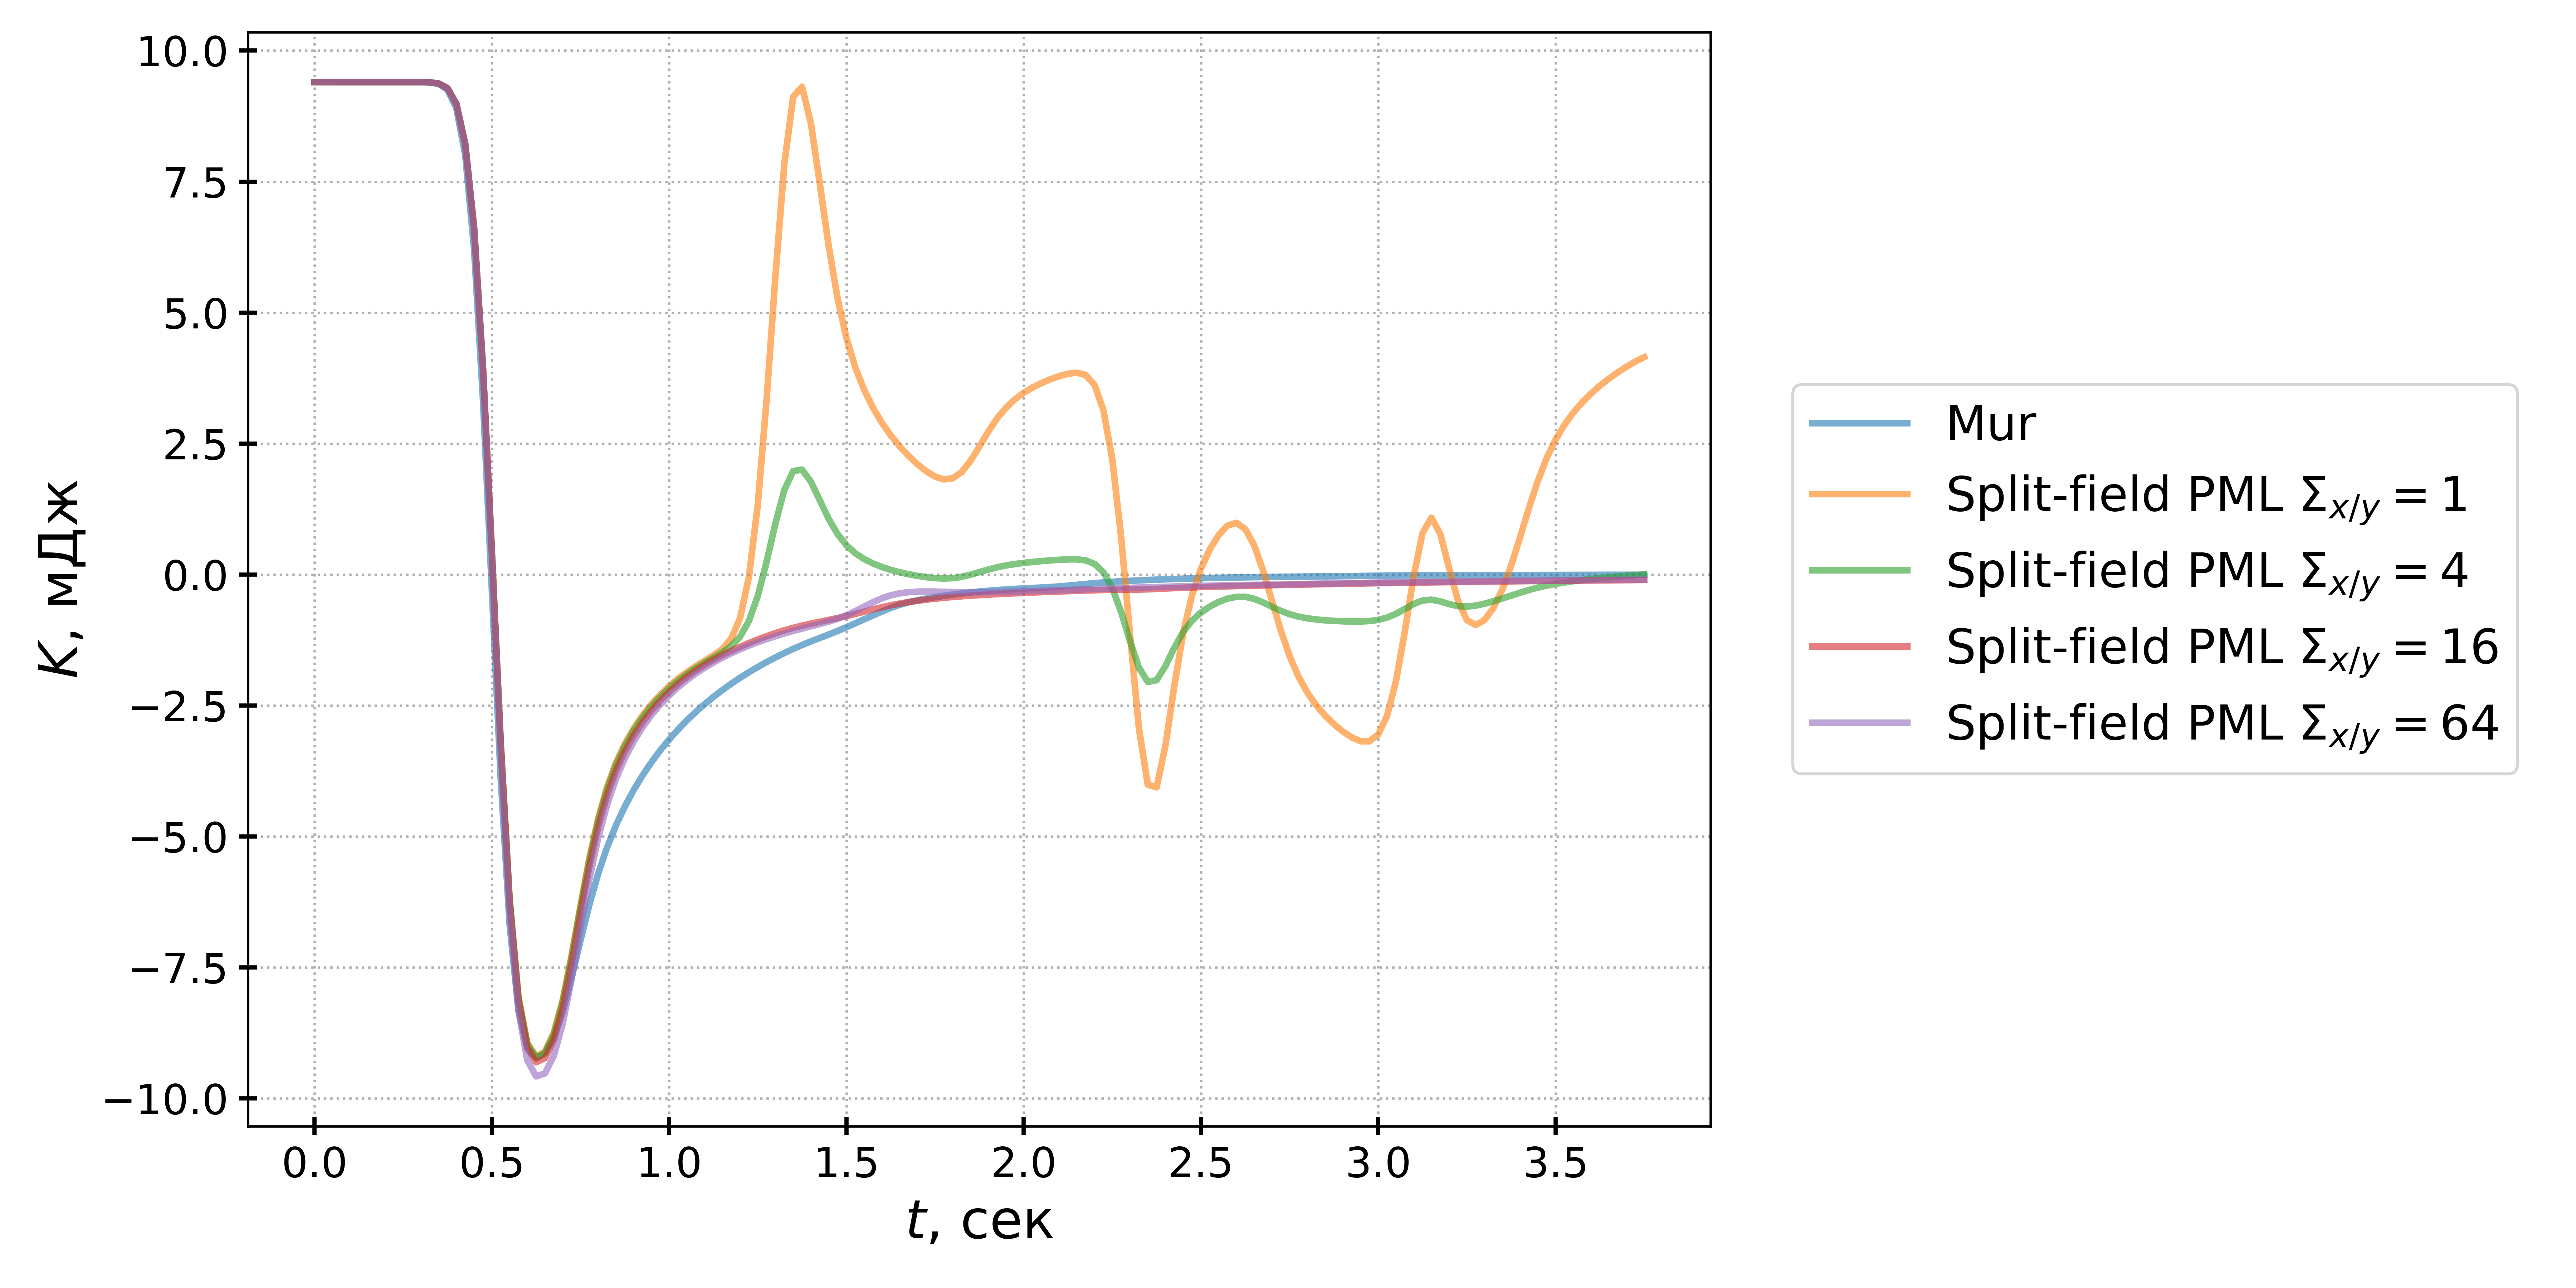
\includegraphics[width=1.0\textwidth]{images/pml/fd_split_field.png}
    \caption{Зависимость кинетической энергии от времени для конечно-разностной реализации поглощающих граничных условий Mur и split-field PML для различных значений параметра $\Sigma_{x/y}$.}
    \label{fig:fd_split_field_pml}
\end{figure}

\subsection{Методы оценки результатов}

%Для оценки эффективности PML и сравнения PML для конечно-разностных и сеточно-характеристических методов предлагается строить график зависимости нормализованного давления от времени, как это делается в \cite{pml-acoustic}. Там же приводится способ получения аналитического решения посредством обратного преобразования Фурье.

%Другой метод оценки идеального затухания состоит в моделировании на в несколько раз большей сетке, и использовании только его центральной части. Таким образом, при выборе достаточно большой сетки и достаточно малого временного промежутка, начальная волна пройдёт полностью через мнимые границы без отражения, а реальная отражённая волна не успеет вернуться, и в итоговом восприятии мы получим идеальное поглощение.
